% Nikolai Nielsens "Fysiske Fag" preamble
\documentclass[a4paper,10pt]{article} 	% A4 papir, 10pt størrelse

\usepackage{Nikolai} 					% Min hjemmelavede pakke
\usepackage[dvipsnames]{xcolor}

% Margen
\usepackage[margin=1.3in]{geometry}

% Max antal kolonner i en matrix. Default er 10
%\setcounter{MaxMatrixCols}{20}

% Hvor dybt skal kapitler labeles?
%\setcounter{secnumdepth}{4}	
%\setcounter{tocdepth}{4}


% Hvilket nummer skal der startes med i sections? (n-1)
%\setcounter{section}{0}	

% Til nummerering af ligninger. Så der står (afsnit.ligning) og ikke bare (ligning)
\numberwithin{equation}{section}

% Header
%\usepackage{fancyhdr}
%\cfoot{\thepage}
%\pagestyle{fancy}

%Titel
\title{% 
	Datalogi for Fysikere 2016/2017, Eksamensprojekt\\
	\large Simulation af to racer af vekselvirkende individer}
\author{Nikolai Plambech Nielsen, LPK331}

\begin{document}

	\selectlanguage{danish}
	
	\clearpage\maketitle
	\thispagestyle{empty}
	\vspace{2cm}
	\begin{figure}[H]
		\centering
		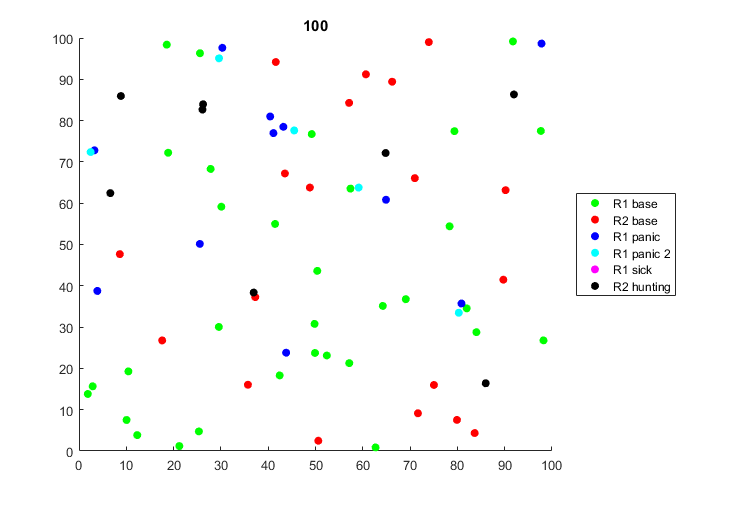
\includegraphics[width=\textwidth]{img/front.png}
	\end{figure}
	\newpage
	\setcounter{page}{1}
	
	\section{Introduktion}
	Dette er en rapport over eksamensprojektet i DatF (Datalogi for Fysikere), 2016/2017. Eksamensprojektet går ud på at simulere en verden, hvor der lever to forskellige racer, der bekriger hinanden. Race 1 fungerer som en slags bytte for race 2, der jæger disse, men som i specifikke tilfælde kan blive dræbt af individer af race 1.0.
	
	Reglerne for simulationen er som følger: Begge racer bevæger sig med konstant hastighed i et tidsrum (race 1 bevæger sig hurtigere end race 2, og i længere tid). Når dette tidsrum er gået, skifter de retning på tilfældig vis, og fortsætter med samme konstante hastighed. Dette er basistilstanden for hver race. For race 1 gælder yderligere:
	\begin{itemize}
		\item Individerne har et synsfelt på $ \pm 90 $\Deg.
		\item Hvis de ser et individ af race 2, inden for en bestemt afstand (kaldet r\_panik), går de i panik, drejer sig 180\Deg og bevæger sig dermed i modsat retning, nu med dobbelt hastighed.
		\item Hvis de ser et individ af race 1, som samtidig er i panik, går de selv i en slags ">sekundær"< panik. De bevæger sig med dobbelt hastighed i en tilfældig retning (og de kan dermed risikere at løbe ind i et race 2 individ).
		\item Hvis et race 2 individ kommer inden for en given radius (mindre end panikradius), og race 1 individet et inden for race 2 individets synsfelt, så bliver race 1 individet syg, hvorefter det bevæger sig med 1.5 gange den normale hastighed i et tidsrum, inden individet bliver transformeret til et race 2 individ.
		\item Hvis et race 2 individ kommer inden for en endnu mindre radius, og race 2 individet kan se race 1 individet, så bliver race 1 individet transformeret med det sammen. Hvis \textit{ikke} race 2 individet kan se race 1 individet, transformeres race 2 individet til et race 1 individ.
	\end{itemize}

	For race 2 gælder
	\begin{itemize}
		\item Individerne har et synsfelt på $ \pm 45 $\Deg.
		\item Hvis et race 2 individ ser et race 1 individ inden for en given radius (større end race 1s panikradius), begynder de at jage dette individ. Hvis der er flere individer, der opfylder dette krav, vælges det individ, der er tættest på.
	\end{itemize}
	Fælles gælder også, at efter et givent tidsrum i en tilstand, for eksempel panik, vil individet gå tilbage til sin basistilstand (ud over for syge race 1 individer, der bliver til race 2 individer efter sygdomsperioden). Hvis et individ ydermere kommer ud til kanten af verden, skal de reflekteres ind igen.
	
	Forholdet mellem afstande er sådan, at 
	\begin{equation*}
		\text{Jage} > \text{Panik} > \text{Sekundær panik} > \text{Syg} > \text{Død}
	\end{equation*}
	Så først vil race 2 begynde at jage race 1, hvorefter race 1 går i panik. Tættere på går eventuelle andre race 1 individer i panik, og endnu tættere på bliver race 1 syg. Aller tættest på transformerer et individ (alt efter om race 2 ser race 1 eller ej).
	
	
	Formålet med denne rapport er at dokumentere projektet. Hvad projektet går ud på, implementering af selve simulationen og dennes regler, brugen af koden samt mit syn på forløbet.
	
	\section{Beskrivelse af programmet}
	Programmet virker ved at have en række matricer, hvori informationerne om hvert individ er dokumenteret. Herunder matricer for position, hastighed, tilstand og lignende. Disse matricer bruges af programmet til at foretage beslutninger om, hvad der skal ske i simulationen. 
	
	Én iteration af simulationen foregår ved, at der først ses på individernes indbyrdes positioner, for at se om deres tilstand skal ændres fra én tilstand til en anden, som beskrevet ovenfor, enten ved at de er inden for en given radius og synsfelt, eller at de har tilbragt et givent tidsrum i tilstanden.
	
	Efter dette tjek opdateres individernes position ud fra deres hastighedsvektorer, ved simpel Eulerintegration:
	\begin{equation*}
		\V{r}(t = t_0+ \ud t) = \V{r}(t=t_0) + \V{v} \ud t
	\end{equation*}
	Når den nye position er udregnet, tjekkes det om nogen individer er nået ud over spillepladen, hvormed deres hastighedsvektor og positionsvektor skal opdateres, således at de reflekteres og forbliver inde på spillepladen.
	
	Efter alle disse ting opdateres grafikken og én iteration er gennemført. Inden første iteration indlæses alle startbetingelser (tilfældig startposition og retning). Når disse er genereret og al relevant data er indlæst startes grafikken med startbetingelserne, og den første iteration påbegyndes.
	
	Denne simulation stopper efter et givent antal iterationer er udført, bestemt af brugeren i starten af programfilen.
	
	\subsection{Sådan køres programmet}
	For at køre programmet skal MATLAB (testet på version R2016a) være installeret på din computer, og du skal have alle programfilerne (de 8\footnote{edgecase.m, init.m, plotter.m, projekt.m, rv.m, statechange.m, time.m \& velupdate.m} filer med endelsen ">.m"<). Når du har sikret dig dette, skal du dobbeltklikke på filen ">projekt.m"<, der er hovedfilen. Dette åbner filen i MATLAB. Når MATLAB er åbnet skal du klikke på knappen ">run"<, der har en grøn trekant, som peger mod højre som ikon (som en play-knap på en DVD eller Bluray afspiller). Se figuren herunder for hjælp.
	\begin{figure}[H]
		\centering
		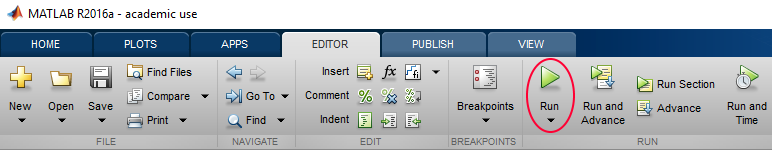
\includegraphics[width=\textwidth]{img/run.png}
		\caption{tryk på knappen ">Run"<.}
		\label{fig:run}
	\end{figure}
	
	Hvis der popper en boks op, som ligner den på figuren herunder, skal du bare trykke på ">change folder"<. Denne popper op fordi MATLAB til at starte med kun kigger i sin startmappe, og når man prøver at køre et program uden fra startmappen, så skal MATLAB lige være sikker på, at man vil skifte til en anden mappe, inden den vil lade dig køre programmet.
	\begin{figure}[H]
		\centering
		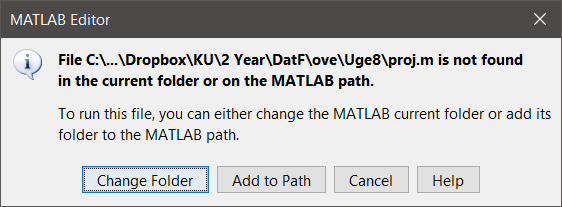
\includegraphics[width=10cm]{img/folder.png}
		\caption{tryk på knappen ">Change Folder"<.}
		\label{fig:folder}
	\end{figure}
	
	Når du har trykket på ">run"< (og eventuelt ">change folder"<) starter simulationen. Efter et kort stykke tid vil der åbnes et vindue der ligner dem i afsnittet ">Eksempel på simulation"<, og simulationen vises i dette vindue.
	
	Hvis du vil ændre på startbetingelserne i programmet, skal du i MATLABs editor ændre på tallene i de linjer, der står op ved toppen af programfilen. Ud fra hver linje står der et procenttegn, efterfulgt af noget tekst, der beskriver, hvad hver linje gør.
	
	\begin{figure}[H]
		\centering
		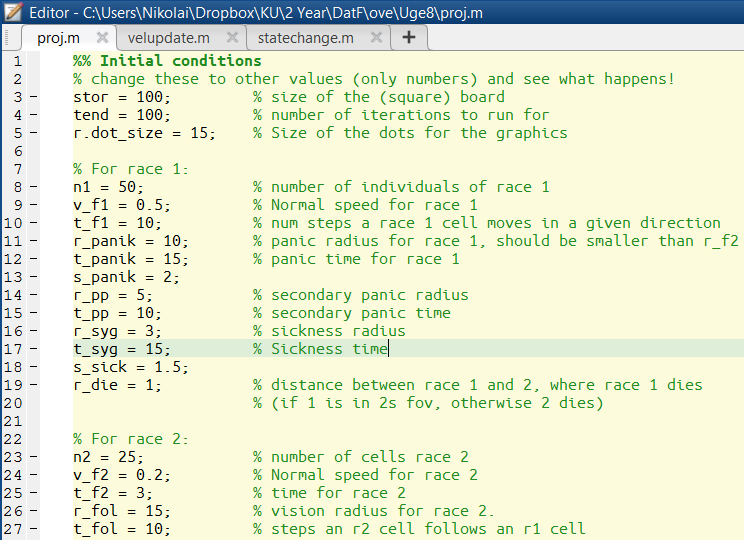
\includegraphics[width=12cm]{img/editor.png}
		\caption{MATLABs editor. Du kan frit ændre på tallene i denne sektion kaldet ">initial conditions"<.}
		\label{fig_editor}
	\end{figure}
	
	\subsection{Begrænsninger}
	Der er selvfølgelig flere forskellige begrænsninger ved denne model, men det kommer helt og aldeles an på, hvad man prøver at modellere. Hvis det er komplekst liv, man prøver at modellere, så er det ikke en særlig realistisk model. For eksempel bør individer måske ikke bare ændre retning diskontinuert til en ny, tilfældig retning. Der bør også være noget acceleration, da overgangen fra basistilstand til panik for race 1 (eksempelvis) medfører en uendelig acceleration, der bestemt ikke er realistisk. Ydermere er det en firkantet spilleplade, hvor individer bare reflekteres som var de lysstråler (indgangsvinklen er lig udgangsvinklen i forhold til fladenormalen). Det er klart den mest enkle måde at gøre det på, men ikke særlig realistisk.
	
	Man kan altid prøve at gøre det mere realistisk, men man er nødt til at lave nogle antagelser og på et eller andet punkt stoppe, så simulationen stadig kan køre i et ordentligt tidsrum.
	
	\newpage
	\section{Eksempel på simulation}
	Herunder vises en simulation der kører i 75 iterationer, og viser startbetingelserne, og så hvert 25. skridt.
	\begin{figure}[H]
		\centering
		\begin{minipage}{0.45\textwidth}
			\centering
			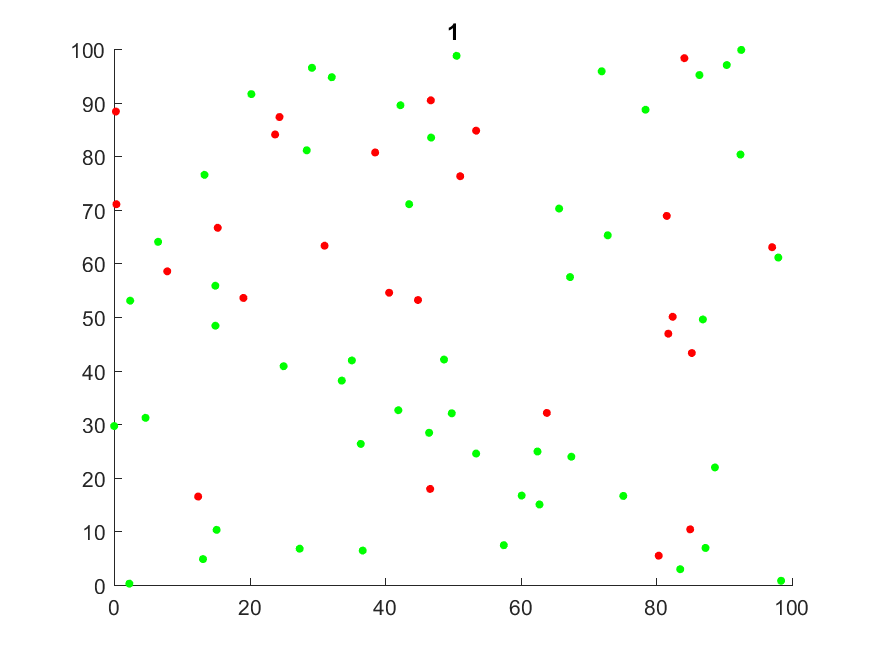
\includegraphics[width=\textwidth]{img/plot1.png}
		\end{minipage}
		\begin{minipage}{0.45\textwidth}
			\centering
			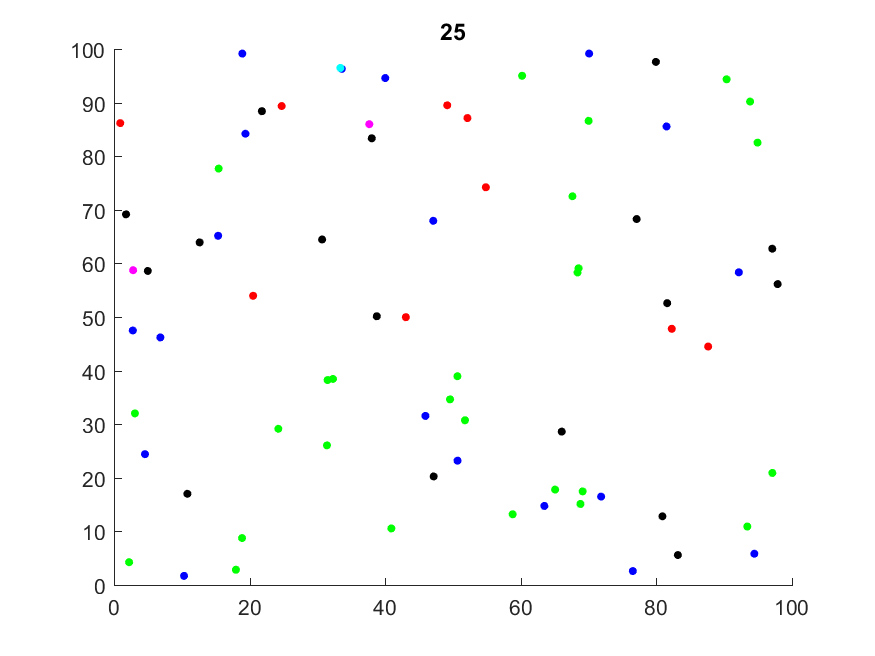
\includegraphics[width=\textwidth]{img/plot2.png}
		\end{minipage}
		\begin{minipage}{0.45\textwidth}
			\centering
			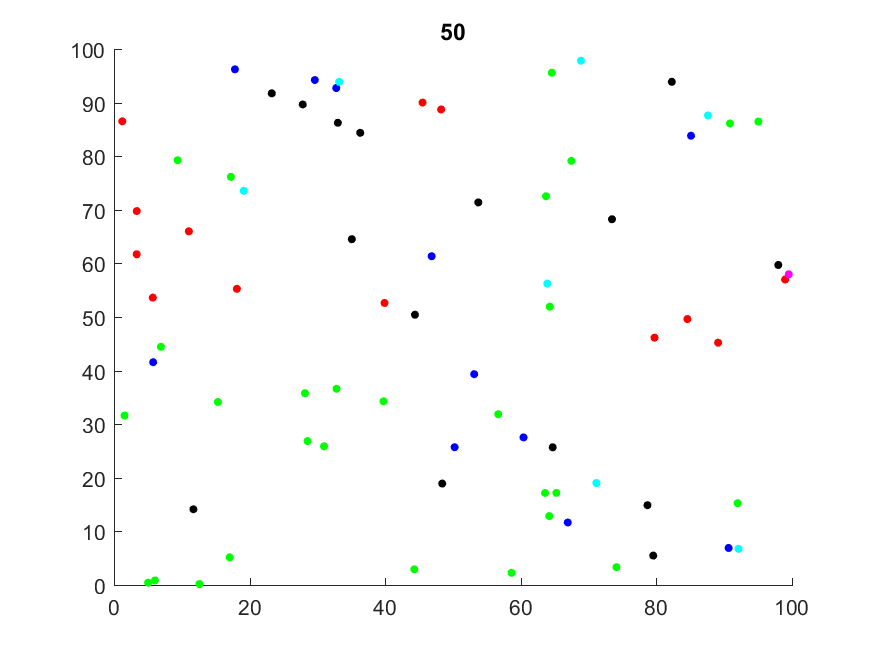
\includegraphics[width=\textwidth]{img/plot3.png}
		\end{minipage}
		\begin{minipage}{0.45\textwidth}
			\centering
			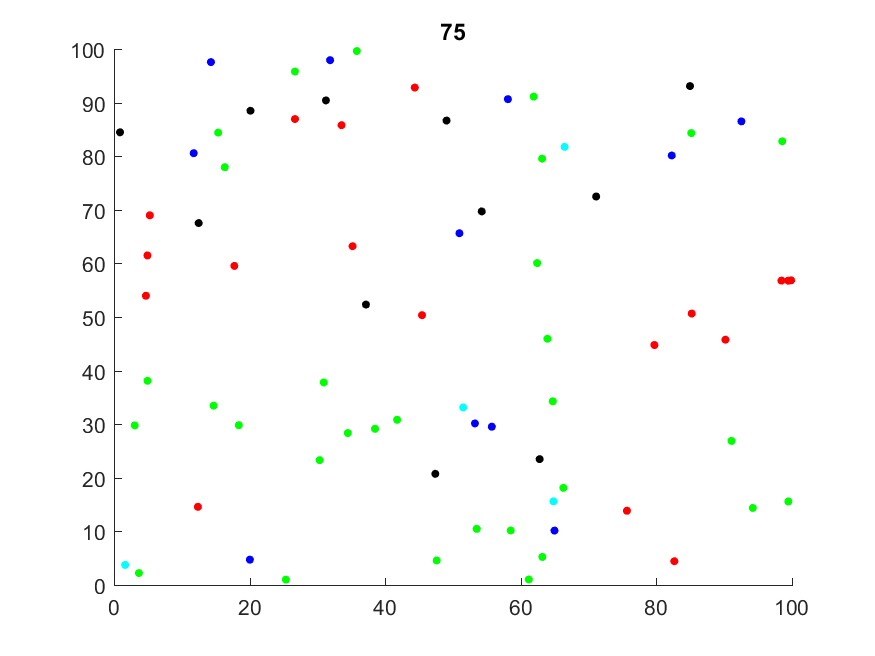
\includegraphics[width=\textwidth]{img/plot4.png}
		\end{minipage}
	\caption{Tidsudvikling af simulationen. Race 1 i \textcolor{green}{basistilstand vises i grønt}, \textcolor{blue}{panik vises i blåt}, \textcolor{cyan}{sekundær panik vises i lyseblåt}, \textcolor{VioletRed}{sygdom vises i lyserødt}. Race 2 individer i \textcolor{red}{basistilstand vises i rødt} og jagt vises i sort.}
	\end{figure}


	\section{Opsummering}
	Jeg synes dette var en rigtig fin opgave, med nok at lave til, at man kunne bruge både sin viden om matematik og fysik, samt programmering. Man kunne implementere metoderne, som vi har fået introduceret i dette kursus, hvilket jeg også har prøvet på. Hen mod slutningen blev det klart sværere at lave alt vektoriseret, hvilket produktet også afspejler. I simulationen er det klart funktionen ">statechange"< der bruger længst computationstid (hvis der ses bort fra plots), og dette er en funktion, der overhovedet ikke er vektoriseret.
	
	Med mere tid ville jeg uden tvivl have vektoriseret denne funktion, samt inkluderet en gui, for at gøre programmet mere brugervenligt (dette kunne dog blive problematisk, når der er så mange knapper der kan skrues på, og ikke ubegrænset plads på skærmen).
	
	Men med den tid vi nu en gang havde, synes jeg det er blevet et rigtig godt produkt, hvor man virkelig har kunnet fordybe sig i det, og selv vælge hvordan og hvorledes det hele skal struktureres og udføres.

\end{document}

